\documentclass[11pt]{article}

\usepackage[utf8]{inputenc}
\usepackage[T1]{fontenc}
\usepackage{lmodern}
\usepackage[margin=1in]{geometry}
\usepackage{amsmath,amssymb,amsthm}
\newtheorem{proposition}{Proposition}
\usepackage{graphicx}
\usepackage{booktabs}
\usepackage{natbib}
\setlength{\bibsep}{0.3ex plus 0.2ex}
\usepackage{multicol}
\usepackage{lineno}
\usepackage{hyperref}
\hypersetup{colorlinks=true,linkcolor=blue,citecolor=blue,urlcolor=blue}
\makeatletter
\g@addto@macro\UrlBreaks{\do\/\do\-\do\.\do\=\do\?\do\&\do\_\do\:}
\makeatother

\title{From Areas to Buildings: Sub-Neighbourhood Fire Risk Concentration and
Physics-Calibrated Consequence Modelling for English Dwellings}

\author{Matthew Reid}
\date{\today}

\begin{document}
\linenumbers
\maketitle

\begin{abstract}
A companion paper established a calibrated, uncertainty-aware framework for
residential fire-risk assessment in England, bounded by two granularity
ceilings: incident geography no finer than the small statistical area (Lower
layer Super Output Area, LSOA), and a consequence simulator that is
mechanistically structured rather than physical. This paper attacks both ceilings and
reports, with equal weight, what was gained and what remains out of reach.
Spatially, London's uniquely fine incident records (90{,}318 dwelling fires at
50\,m resolution, 2009--2024) show that within an average LSOA the top decile of
inhabited cells holds 83\% of dwelling fires against 59\% under a
dwelling-density null; evaluated out-of-sample, cell-level targeting reaches
dwellings with 4--6$\times$ the fire rate of LSOA-level targeting, lifting a
smoke-alarm visit programme above break-even where area-level targeting is not
close. At the individual-building scale, the record subset carrying full
building identifiers (33{,}498 care homes, hostels, hotels, and student halls) supports
a calibrated per-building fire model exhibiting 11-fold rate heterogeneity, and
identifies a building's false-alarm burden as a stable, measurable
alarm-reliability observable that independently predicts subsequent fires.
Mechanistically, we construct a zone-model physics engine (NIST CFAST) over the
companion framework's building archetypes --- construction-era-derived boundary
materials, design fires keyed to the national ignition-source distribution, and
standardised tenability criteria --- and calibrate its physical parameters
against the observed English spread margins using a Bayesian
calibration-with-discrepancy formulation over a 5{,}040-point zone-model design
bank. The calibrated physics reproduces all 22 observed spread margins to within
$\approx$0.001 absolute probability (17 of 22 inside their posterior-predictive
intervals), but aggregate incident margins identify
only one physical parameter (effective door-openness, sharpened by $\approx$50\% and
shifted to 0.72 of its design value); the remaining fire-growth and material
parameters are returned prior-dominated, an identifiability ceiling we
characterise rather than obscure. The path through that ceiling --- timed,
scenario-resolved calibration targets --- defines the data-access agenda that
building-resolved fire-risk modelling now requires.
\end{abstract}

\section{Introduction}
\label{sec:intro}

The companion paper to this work (Reid, in preparation --- developed on the
same open-data infrastructure of English incident statistics
\citep{mhclg2026firestats}, the EPC register, and census/deprivation data)
recast UK fire risk assessment --- the periodic, checklist-based practice of
the PAS~79 / Building Safety Act regime \citep{pas79_1_2020,bsa2022} --- as
Bayesian inference: a calibrated posterior over ignition, spread, and
consequence for every English small area, validated out-of-time, and coupled to
a decision layer that allocates prevention resources by expected benefit. Two
ceilings bounded that contribution, both imposed by the available data rather
than the method.

The first is \emph{geographic}. National incident records resolve dwellings
only to the Lower layer Super Output Area (LSOA, $\approx$650 households), so
the framework's risk surface --- and any targeting built on it --- is constant
within each area. If fire risk is strongly concentrated \emph{within} areas,
area-level targeting forfeits value invisibly.

The second is \emph{mechanistic}. The companion framework estimates
consequences with a transparent stochastic simulator whose structure mirrors
fire mechanisms but whose quantities are assumption-driven; it is
mechanistic in structure, not in physics. Fire engineering possesses real physics ---
zone and field models with decades of validation --- but these have never been
\emph{statistically calibrated} against national incident outcomes, so their
parameters carry order-unity uncertainty for exactly the building stock that
population-scale risk modelling addresses.

This paper attacks both ceilings with the two finest-grained public data
resources in England, and reports symmetric verdicts. Section~\ref{sec:london}
uses London's uniquely fine incident geography to measure sub-LSOA risk
concentration and its decision value. Section~\ref{sec:buildings} exploits the
record subset carrying full building identifiers to fit the first calibrated
per-building fire model in this programme, and introduces false-alarm burden as
a measurable alarm-reliability observable. Sections~\ref{sec:engine}
and~\ref{sec:calibration} construct a zone-model physics engine over the
companion framework's archetypes and calibrate it against observed spread
margins with a Kennedy--O'Hagan discrepancy formulation \citep{kennedy2001},
establishing precisely which physical parameters English incident data can and
cannot identify. Section~\ref{sec:discussion} draws the programme-level
conclusion: the marginal value of finer data is now quantified on both axes,
and the identified bottleneck is timed, scenario-resolved outcomes.

Throughout, we hold to the companion framework's reporting discipline: every
result is out-of-sample or posterior-predictive checked; every null,
identifiability failure, and numerical limitation is reported with the same
prominence as the positive results.

\section{Sub-LSOA concentration: what finer geography is worth}
\label{sec:london}

\subsection{Data and design}

The London Fire Brigade (LFB) is the one English fire service publishing
incident-level records with sub-LSOA geography \citep{lfb_incidents}: dwelling
incidents carry a British National Grid coordinate rounded to 50\,m
($\approx$2{,}500\,m$^2$ cells). We take 90{,}318 primary dwelling fires
(fiscal 2009--2024) on this grid. Exposure comes from the Energy Performance
Certificate (EPC) register \citep{epcregister2025}: 2.60\,million London
dwellings positioned by their open Unique Property Reference Number (UPRN)
coordinates and rounded to the same grid --- 307{,}146 inhabited cells across
5{,}135 LSOAs, so fires and dwellings share one geography. EPC covers
$\approx$74\% of London stock; the 14\% of fires falling in cells with no EPC
dwelling are excluded from observed and null alike, which (with the 50\,m
rounding itself) makes every concentration estimate below conservative.

Concentration must be measured against the right null: dwelling density is
itself uneven, and rare-event counts concentrate by chance. Per LSOA we
therefore compare the observed concentration to a \emph{dwelling-density
multinomial null} --- the LSOA's fires redistributed across its cells with
probability proportional to dwellings per cell, 400 draws per LSOA --- and
report the excess.

\subsection{Result: risk is concentrated well beyond density}

\begin{table}[htbp]
  \centering
  \caption{Within-LSOA fire concentration, fire-weighted mean over 5{,}135
  London LSOAs. The null already concentrates (uneven dwelling density plus
  small-count noise); the signal is the excess.}
  \label{tab:concentration}
  \small
  \begin{tabular}{@{}lccc@{}}
    \toprule
    Metric & Observed & Density null & Excess \\
    \midrule
    Top-10\%-of-cells fire share & \textbf{0.831} & 0.591 & $+$0.240 \\
    Gini across cells            & 0.880 & 0.762 & $+$0.117 \\
    \bottomrule
  \end{tabular}
\end{table}

Within an average LSOA, the top tenth of inhabited cells holds 83\% of the
fires --- 24 points more than dwelling density and sampling noise explain
(Table~\ref{tab:concentration}, Figure~\ref{fig:concentration}). Sub-LSOA
structure is real, large, and invisible to any national model --- the built
environment's analogue of the ``law of concentration'' long documented for
crime at place \citep{weisburd2015}.

\begin{figure}[htbp]
  \centering
  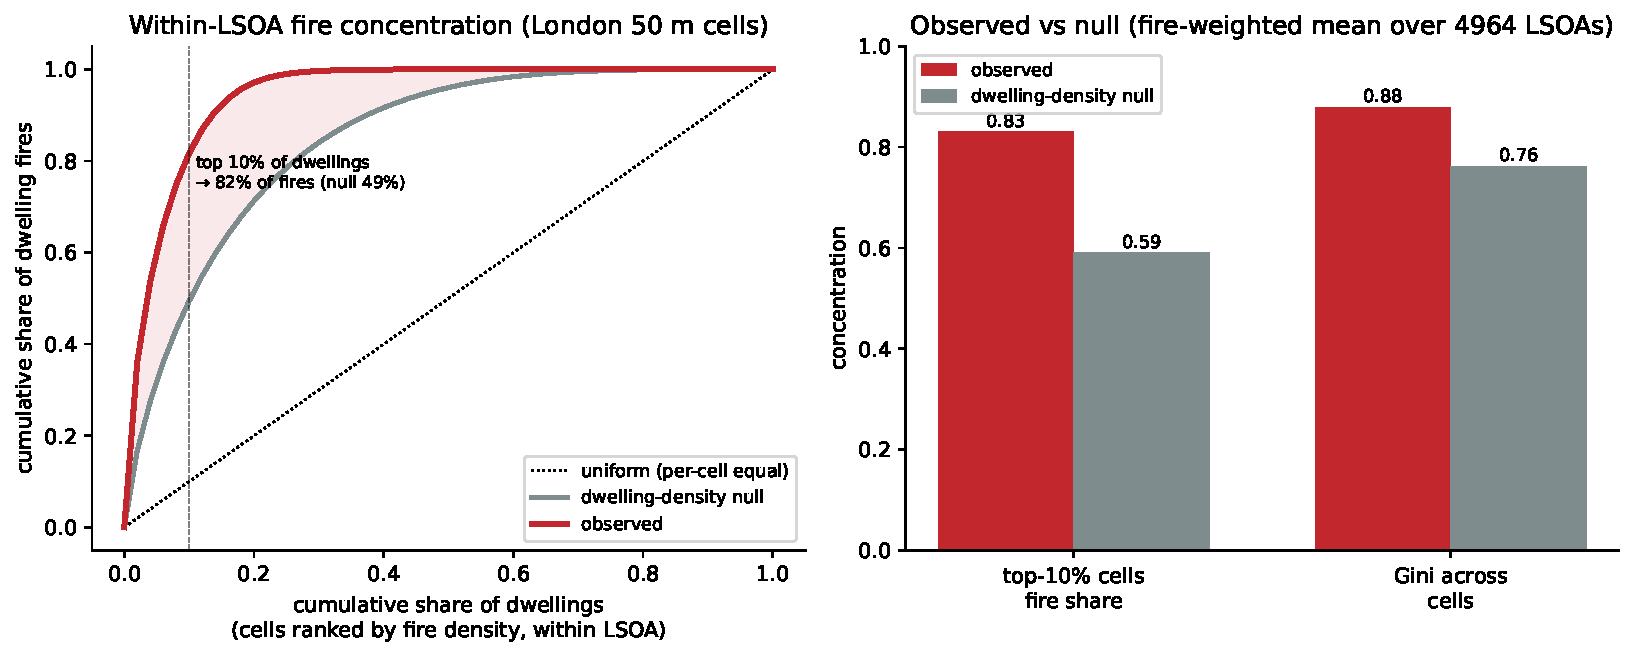
\includegraphics[width=0.72\linewidth]{figures/concentration.pdf}
  \caption{Within-LSOA Lorenz curves over 50\,m cells: observed fire
  concentration vs the dwelling-density multinomial null.}
  \label{fig:concentration}
\end{figure}

\subsection{Decision value, out of sample}

Concentration only matters if it is \emph{predictable}. We price it with the
companion framework's prevention economics (a \pounds55 home safety visit;
casualty and property channels; ten-year present value) under strict temporal
separation: 50\,m cells are ranked on 2009--2020 fire history using
empirical-Bayes (EB) shrunk rates. Cell $i$'s latent rate carries a Gamma prior
$\lambda_i \sim \mathrm{Gamma}(r,\, r/\bar\lambda_{\ell(i)})$ around its
LSOA mean $\bar\lambda_{\ell(i)}$, so observing $f_i$ fires over $d_i$
dwellings and $T$ years gives the conjugate posterior mean
\begin{equation}
  \hat\lambda_i \;=\;
  \frac{r + f_i}{\,r/\bar\lambda_{\ell(i)} + d_i T\,}
  \;=\; w_i\, \frac{f_i}{d_i T} \;+\; (1-w_i)\,\bar\lambda_{\ell(i)},
  \qquad
  w_i = \frac{d_i T}{\,d_i T + r/\bar\lambda_{\ell(i)}\,},
  \label{eq:eb}
\end{equation}
a precision-weighted compromise between the cell's own noisy empirical rate and
its neighbourhood mean --- exactly the machinery that ignores the
single-dwelling-cell noise a raw ranking rewards. The shape $r\approx0.14$
(strong within-LSOA heterogeneity, hence weak shrinkage for well-observed
cells) is estimated by maximising the negative-binomial marginal likelihood
implied by the Gamma mixing. Every dwelling selected under a fixed London visit
budget is scored at its cell's \emph{realised 2021--2024} rate. LSOA-level targeting
--- the national model's ceiling --- assigns every dwelling its area-average
rate.

\begin{table}[htbp]
  \centering
  \caption{Out-of-sample value of sub-LSOA targeting (ranked 2009--2020,
  scored on realised 2021--2024 rates). The oracle column uses perfect
  foresight of the scoring window and bounds the achievable multiplier; the gap
  between it and the EB column is the share of apparent concentration that is
  noise.}
  \label{tab:cellvalue}
  \small
  \begin{tabular}{@{}rcccc@{}}
    \toprule
    London budget & LSOA \pounds/\pounds & Cell-EB \pounds/\pounds &
    Rate multiplier (EB) & (oracle) \\
    \midrule
    10{,}000  & 0.33 & \textbf{1.88} & \textbf{5.7$\times$} & 11.3$\times$ \\
    25{,}000  & 0.27 & 1.34 & 5.0$\times$ & 9.0$\times$ \\
    50{,}000  & 0.22 & 1.05 & 4.7$\times$ & 7.5$\times$ \\
    100{,}000 & 0.19 & 0.82 & 4.2$\times$ & 6.1$\times$ \\
    \bottomrule
  \end{tabular}
\end{table}

Cell-level targeting reaches dwellings with four to six times the fire rate of
LSOA-level targeting (Table~\ref{tab:cellvalue}, Figure~\ref{fig:targeting}),
enough to carry the smoke-alarm channel alone above break-even
(\pounds1.88/\pounds1 at 10{,}000 visits) where area-level targeting is not
close. Because no cell-level occupancy or alarm-ownership data exist, every
cell shares national consequence parameters: the multiplier is driven purely by
fire-rate concentration, and cell-level vulnerability data could only widen it.

\subsection{Where the budget goes}

The 10{,}000-visit policy selects 1{,}948 cells spread across 32 of London's 33 local authorities (only
the City of London, with its tiny dwelling stock, receives none) --- targeted,
not monolithic --- with the densest cluster in inner
south London (Southwark and Lambeth around Elephant \& Castle, Kennington and
Peckham). Table~\ref{tab:boroughs} names the allocation, and its final column
is itself an out-of-sample check: the dwellings the policy selects on
2009--2020 history go on to burn at 23--48 fires per 1{,}000 dwelling-years in
2021--2024 --- an order of magnitude above the London average --- in every
borough on the list. Figure~\ref{fig:map} shows the geography as an
estimate-vs-realised grid over the same selected cells in both the training
and held-out windows: the visual form of the validation, with the cells that
received visits but recorded no subsequent fire kept explicitly in view.

\begin{table}[htbp]
  \centering
  \caption{Borough allocation of the 10{,}000-visit London policy (top ten by
  budget share). The final column scores the selected cells at their realised
  out-of-sample rate: the policy's choices burn at $\sim$10$\times$ the London
  dwelling average in the scoring window it never saw.}
  \label{tab:boroughs}
  \small
  \begin{tabular}{@{}lrrrcc@{}}
    \toprule
    Borough & Cells & Visits & \% budget &
    EB rate$^{\dagger}$ & Realised 2021--24 rate$^{\dagger}$ \\
    \midrule
    Southwark     & 153 & 895 & 9.0\% & 53.6 & 47.8 \\
    Hackney       & 131 & 791 & 7.9\% & 46.9 & 33.5 \\
    Brent         & 119 & 563 & 5.6\% & 43.2 & 29.8 \\
    Lambeth       &  88 & 521 & 5.2\% & 42.8 & 27.8 \\
    Tower Hamlets &  77 & 506 & 5.1\% & 44.2 & 31.1 \\
    Lewisham      &  92 & 488 & 4.9\% & 42.8 & 22.5 \\
    Haringey      &  90 & 474 & 4.7\% & 42.0 & 26.9 \\
    Greenwich     & 108 & 454 & 4.5\% & 43.7 & 34.7 \\
    Croydon       & 101 & 421 & 4.2\% & 42.2 & 22.6 \\
    Camden        &  71 & 408 & 4.1\% & 44.7 & 31.9 \\
    Rest (22 boroughs) & 918 & 4{,}479 & 44.8\% & 43.5 & 29.6 \\
    \bottomrule
  \end{tabular}

  \smallskip
  {\footnotesize $^{\dagger}$dwelling fires per 1{,}000 dwelling-years.}
\end{table}

\begin{figure}[htbp]
  \centering
  \includegraphics[width=\linewidth,height=0.58\textheight,keepaspectratio]{figures/map_targeting.pdf}
  \caption{Estimate vs realised for the same 1{,}948 policy-selected cells, in
  and out of sample, on identical extents and one shared log colour scale.
  Columns: the empirical-Bayes (EB) estimate the policy machinery produces
  (left) against the realised raw counted rate (right). Rows: the 2009--2020
  training window (top) and the held-out 2021--2024 window (bottom).
  The intended reading: the estimate column is spatially stable across
  windows --- the same inner-south/east clusters, moderated saturation ---
  while the realised column runs hotter and patchier, the signature of raw
  small-denominator rates. The bottom row is the out-of-sample validation in
  visual form: the 2009--20 selection anticipates where the 2021--24
  concentration falls. Honesty is kept in frame: grey cells in the
  bottom-right panel are selected cells with \emph{zero} realised fires in
  2021--24 --- 1{,}172 of 1{,}948 (60\%), as expected when targeting rare
  events over a four-year window; the policy's value is carried by the rates
  of the cells that do burn (Tables~\ref{tab:cellvalue}
  and~\ref{tab:boroughs}). The colour scale is floored at 5 fires per 1{,}000
  dwelling-years (palest colour = at or below floor, including EB estimates in
  zero-fire LSOAs) and capped at the realised-panel 99th percentile. Basemap
  \copyright\ CARTO, \copyright\ OpenStreetMap contributors.}
  \label{fig:map}
\end{figure}

\begin{figure}[htbp]
  \centering
  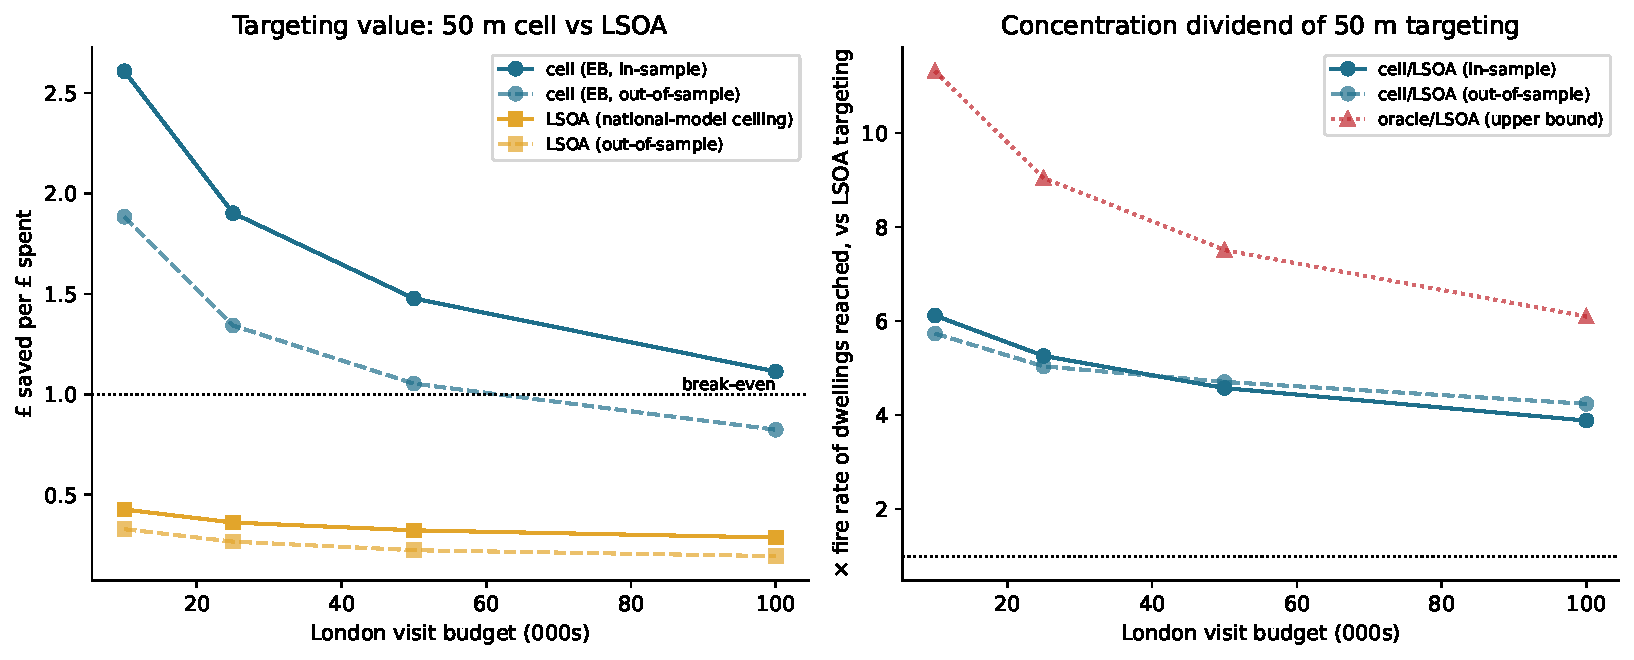
\includegraphics[width=0.8\linewidth]{figures/targeting.pdf}
  \caption{Cumulative preventable-risk capture and \pounds/\pounds by targeting
  policy and budget, out of sample.}
  \label{fig:targeting}
\end{figure}

\section{Building-resolved inference: the identified-building slice}
\label{sec:buildings}

For most dwellings LFB redacts precise location, but \emph{other-residential}
buildings --- care homes, nursing and retirement homes, hostels, hotels,
student halls --- retain their full UPRN: a building-identified incident panel
of 33{,}498 buildings, 5{,}686 fires and 85{,}676 false alarms over sixteen
years. These are precisely the highest-consequence occupancies of the companion
framework's simulation results, where mobility rather than detection binds
evacuation.

\subsection{A calibrated per-building fire model}

Building $b$'s fires follow
$y_b \sim \mathrm{Poisson}(\lambda_b E_b)$ over its active-window exposure
$E_b$, with $\lambda_b \sim \mathrm{Gamma}(k,\, k/\mu)$ across the stock ---
marginally negative binomial, with the population mean $\mu$ and shape $k$
fitted by maximum marginal likelihood and each building's posterior rate given
conjugately by $\mathbb{E}[\lambda_b \mid y_b] = (k + y_b)/(k/\mu + E_b)$;
covariate and temporal extensions replace $\mu$ with
$\exp(\mathbf{x}_b^{\top}\boldsymbol\beta)$ and are sampled by NUTS with the
same convergence gates as the companion paper. This model is well calibrated at
the individual-building level: training on
2009--2022 and predicting 2023--2024 fires for the 3{,}944 buildings active in
both windows gives a randomised probability-integral-transform
Kolmogorov--Smirnov distance of 0.024 --- matching the area-level national
model's calibration quality, but per building. Reporting discipline requires
the null comparison: a pooled population-rate model achieves the same PIT--KS
(0.024), with the building-history model ahead only on log-score
($+0.005$/building-year) --- fires are rare enough per building that borrowing
a building's own history sharpens ranking more than marginal calibration. Heterogeneity is strong (Gamma
shape 0.63): the 99th-percentile building's rate is eleven times the median
(0.345 vs 0.032 fires/year). Building type carries clean structure: relative
to retirement homes (the most regulated, lowest-rate class), nursing/care homes
run 1.59 [1.44, 1.75], hostels 1.96 [1.80, 2.15], hotels 2.14 [1.92, 2.38] and
student halls 2.74 [2.46, 3.07] --- transient occupancy costs a factor of two
to three. Within the care-home subset joinable to the regulator's register (a sparse
join --- only $\sim$1{,}000 buildings match a Care Quality Commission
record), bed count has no detectable effect (rate ratio 0.99 [0.90, 1.10] per
doubling):
larger homes are not proportionally more fire-prone, consistent with fire-safety
systems scaling with size.

\subsection{False-alarm burden as an alarm-reliability observable}

The panel records fifteen false alarms per fire, and a building's false-alarm
burden is a \emph{stable property}: its rate correlates at Spearman 0.33
($n=5{,}529$, $p\approx10^{-141}$) across two independent eight-year halves.
The companion framework posits alarm reliability as a latent building attribute
observed by no public dataset; this is, to our knowledge, its first direct
public observable. It also carries predictive signal: controlling for a
building's own prior fire rate (itself the strongest predictor, rate ratio 1.28
[1.21, 1.36] per SD) and building type, prior false-alarm burden independently
predicts subsequent fires at 1.07 [1.01, 1.14] per SD. The effect is modest and
its interval sits just above one --- fires are rare per building --- but the
direction is consistent: buildings whose alarm systems misfire more burn more
(Figure~\ref{fig:carehome}).

\begin{figure}[htbp]
  \centering
  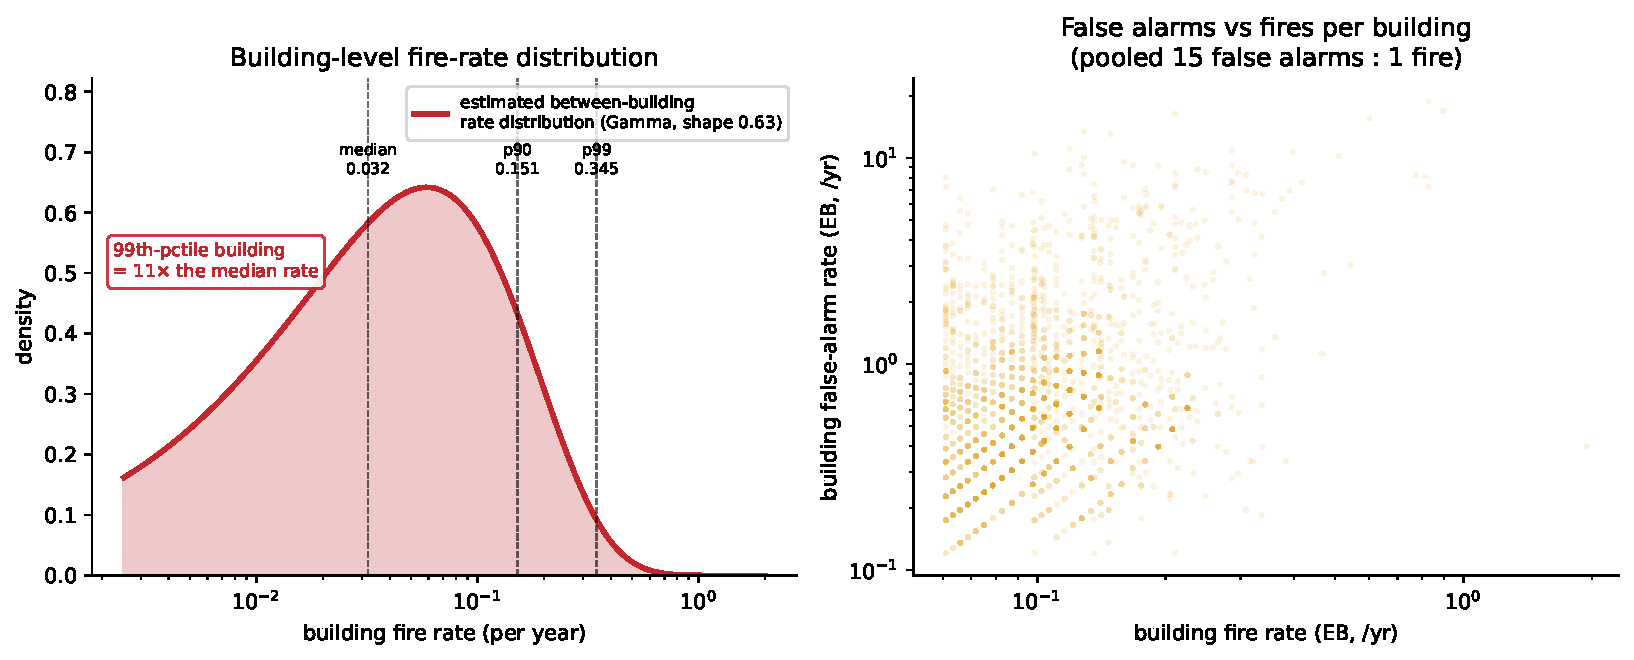
\includegraphics[width=0.9\linewidth]{figures/carehome_rates.pdf}
  \caption{Building-level fire-rate distribution (empirical-Bayes posteriors)
  and false-alarm persistence across independent halves of the record.}
  \label{fig:carehome}
\end{figure}

\subsection{Why a false-alarm burden might predict fires}
\label{sec:buildings:famech}

A predictive link from nuisance alarms to real fires is not mechanically
obvious, and its novelty as a reliability observable is only as useful as the
mechanisms it can stand in for. We set out the candidate pathways as testable
hypotheses, because they carry different implications and the current panel can
separate them only partially.

\emph{(a) Maintenance state.} Nuisance activations are the visible tail of a
poorly maintained or mis-sited detection system: dust- and insect-fouled
chambers, heads past their service life, or the wrong sensor type sited near
kitchens and bathrooms. On this reading the false-alarm rate is a proxy for
detection-system upkeep, and upkeep correlates with the broader fire-safety
regime of the building. \emph{(b) Electrical-fault correlation.} Failing or
overloaded wiring, ageing distribution boards, and degraded appliances generate
spurious detector triggers (transients, arcing, overheating) and are themselves
a leading ignition mechanism, so the false-alarm burden and the genuine
ignition hazard share a common physical cause. \emph{(c) Occupancy intensity and
behaviour.} Heavy cooking, smoking and vaping loads, and high transient
throughput drive both nuisance activations and ignition exposure; here the
false-alarm rate indexes how hard the building is used rather than any fault in
the building itself --- the same axis along which the type effects run
(student halls and hostels highest). \emph{(d) Alarm fatigue.} Repeated false
alarms lead occupants and staff to silence, cover, or disconnect devices and to
discount activations, converting nominal detection into effective non-detection
at the real event. This pathway is the most consequential and the most
actionable: it is a documented operational concern of fire and rescue services,
and it predicts that a building's false-alarm history should degrade outcomes
\emph{conditional} on nominal alarm presence --- exactly the population the
per-building model already conditions on.

These mechanisms are not exclusive, and the present data cannot cleanly
apportion them. Mechanisms (a), (b) and (d) all predict the sign we observe ---
higher false-alarm burden, higher subsequent fire rate --- while (c) predicts it
too but attributes the association to occupancy load rather than to any alarm
property; the type and prior-rate controls in the per-building model absorb some
but not all of that confound. What the panel \emph{cannot} do is distinguish a
detector that misfires because it is broken (a, b) from one that misfires
because the building is used intensely (c) from one whose misfiring later causes
it to be disabled (d). One field already collected by services would go most of
the way: the false-alarm \emph{cause code} (recorded on the incident return ---
e.g.\ cooking fumes, faulty apparatus, malicious, contractor activity)
separates behavioural nuisance from apparatus fault, and a good-intent-versus-
apparatus split would let mechanism (b) be tested directly against (a) and (c).
Joined to the disablement and silencing records some services log, it would also
isolate the alarm-fatigue channel (d). Absent those fields we report the
association and its stability as an observable, and leave the mechanism as the
next question the data can answer.

\section{A physics engine over the archetypes}
\label{sec:engine}

The companion framework's consequence simulator is mechanism-informed: right
structure, assumed quantities. We replace the assumed quantities with zone-model
physics. NIST CFAST \citep{cfast2021,cfastvv2021} solves the two-zone conservation
equations per compartment --- layer temperatures, interface height, species,
vent flows --- in seconds per multi-room scenario, which makes Monte Carlo
physics economically feasible where field models are not.

The engine (built from CFAST v7 source and reproducing NIST's shipped
verification case before use) translates each archetype graph into CFAST
geometry: rooms, corridors, stairs and their door/window vents, with
compartment-boundary thermal properties derived per construction era by
collapsing real multi-layer wall build-ups --- as recorded in the EPC
register's construction descriptions --- to effective single-layer conduction
properties. Design fires are $t^2$ curves keyed to the national
ignition-source distribution with peak heat-release rates (HRR) and yields from the
SFPE handbook literature \citep{tewarson2016}; the battery/charger class ---
the fastest-rising ignition source in English dwellings --- is carried with a
deliberately wide prior reflecting its unsettled experimental base. Tenability
uses the standardised fractional-effective-dose criteria \citep{iso13571}
computed natively by CFAST.

Two behaviours of the engine matter downstream. First, when every door on a
fire's escape route samples shut, the sealed compartment network has no
pressure relief and the stiff-ODE solver halts: this is a \emph{physical
regime} (a contained fire), and we treat such runs as right-censored
observations --- no untenability within the window --- rather than failures,
reclaiming what would otherwise be 63\% of draws. A fixed-flow mechanical
leakage vent was tested as the alternative and does \emph{not} rescue the
sealed regime (0 of 12 vented runs converge at any tested flow), so censoring
stands; a second execution pass re-ran the multi-storey house and HMO
archetypes after an internal-stair geometry correction, converging at 49\%
under a tighter wall-clock budget. Second, tall stair shafts (24 storeys with low door-openness draws,
benchmarked against the documented Grenfell Tower stair timeline
\citep{grenfell2019phase1}) do not converge at all: the two-zone
assumption's known limit, characterised here and excluded from calibration
rather than smoothed over.

\section{Bayesian calibration against 451{,}172 fires}
\label{sec:calibration}

\subsection{Design, emulator, and formulation}

We calibrate six physical multipliers $\theta$ (fire-growth rate, peak heat
release, battery-class heat release, door-openness, boundary conductivity, soot
yield; 1.0 = design value) against the observed English spread margins ---
P(spread beyond room) and P(beyond floor) by archetype, alarm state, and time
of day, from the companion framework's 451{,}172 record-level dwelling fires.
CFAST cannot run inside a sampler, so we sweep $\theta$ over Latin-hypercube
design of 5{,}040 points (2{,}917 usable draws after excluding timeouts and
solver crashes whose fire compartment was not sealed; 6{,}563 executions in
total across two passes, $\approx$3.5\,h at nine-way parallelism) and fit a
bagged gradient-boosted emulator on the bank --- chosen over a Gaussian process
because the spread response is a sharp threshold-shaped function of
door-openness and fire development. Out-of-design validation: holdout area under
the receiver-operating-characteristic curve (AUC) 0.977 (beyond-room) and
0.985 (beyond-floor), degrading only to 0.946/0.943 on a held-out
high-growth extrapolation corner, and robust to the spread-threshold choice.
Calibration follows \citet{kennedy2001}. Their framework (KOH) models a field
observation as
\begin{equation}
  y \;=\;
  \underbrace{f(\boldsymbol\theta)}_{\text{simulator at physical }\boldsymbol\theta}
  \;+\;
  \underbrace{\delta}_{\text{model discrepancy}}
  \;+\;
  \underbrace{\varepsilon}_{\text{observation noise}},
  \label{eq:koh-canonical}
\end{equation}
and its power is in keeping the three terms distinct. $f(\boldsymbol\theta)$ is
the simulator run at physical parameters $\boldsymbol\theta$ --- here the
emulated zone-model physics $\mathrm{logit}\,\eta(\boldsymbol\theta,a)$.
$\delta$ is the \emph{model discrepancy}: the systematic gap between the
best-fitting simulator run and reality that persists even at the true
$\boldsymbol\theta$, because the model itself is incomplete --- missing physics,
the collapse of a real dwelling to a room--corridor--stair archetype, the
two-zone idealisation. $\varepsilon$ is observation-and-sampling noise: here the
binomial fluctuation of a spread margin estimated from a finite count $n_c$ of
fires. The consequence of the decomposition is the whole reason to pay its cost.
Omit $\delta$ and the fit must still be achieved, so the physical parameters
$\boldsymbol\theta$ are driven to absorb the model's structural error; they then
land at values that reproduce the data but no longer mean what they physically
should --- confidently wrong physics. Include $\delta$ and $\boldsymbol\theta$
retains its physical interpretation, but at a price: $\delta$ and
$f(\boldsymbol\theta)$ compete to explain the same residual, so identifiability
weakens and the data sharpen $\boldsymbol\theta$ only where its signature cannot
be mimicked by discrepancy. That trade --- interpretability bought with
identifiability --- is exactly the one this calibration makes, and
Section~\ref{sec:calibration:identify} measures how much of each it buys.
Each observed margin cell $c$ ---
an (archetype $a_c$, alarm state $k_c$, time-of-day $\tau_c$) combination with
$n_c$ fires and $y_c$ spread events --- is modelled as
\begin{align}
  y_c &\;\sim\; \mathrm{Binomial}\big(n_c,\, p_c\big),
  \label{eq:koh-lik}\\
  \mathrm{logit}\, p_c &\;=\;
  \mathrm{logit}\, \eta\big(\boldsymbol\theta,\, a_c\big)
  \;+\; \beta_0
  \;+\; \beta_{\mathrm{alarm}}[k_c]
  \;+\; \beta_{\mathrm{night}}\, \tau_c
  \;+\; \delta_{a_c} ,
  \qquad \delta_{a} \sim \mathcal{N}(0, \sigma_\delta^2),
  \label{eq:koh}
\end{align}
where $\eta(\boldsymbol\theta, a)$ is the emulator's physics prediction of the
spread probability under parameters $\boldsymbol\theta$ --- evaluated, for
sampler efficiency, through a quadratic response surface fitted to the emulator
over the design box in $\log\boldsymbol\theta$ (with $\boldsymbol\theta$
clipped to that box), the emulator's bootstrap-ensemble spread folding into
$\delta$ --- the behavioural terms carry the detection-and-intervention
gradient occupant-free physics cannot produce, and $\delta_{a}$ is the
Kennedy--O'Hagan model discrepancy, indexed by \emph{archetype} and outcome
(one level per archetype rather than per cell, so the discrepancy cannot
absorb the alarm/time gradients it sits alongside) with
$\sigma_\delta \sim \mathrm{HalfNormal}(0.5)$ per outcome. The physical
multipliers are log-normal about their design values,
$\theta_j = e^{\zeta_j}$, $\zeta_j \sim \mathcal{N}(0, \sigma_j^2)$ with the
prior widths of Table~\ref{tab:theta}, and the joint posterior over
$(\boldsymbol\zeta, \beta_0, \boldsymbol\beta, \boldsymbol\delta)$ is sampled
by the No-U-Turn Sampler (four chains, 1{,}000 warmup + 1{,}000 draws, all
$\hat{R}=1.00$, no divergences). Equation~\eqref{eq:koh} also \emph{displays}
the identifiability ceiling: a global shift in
$\mathrm{logit}\,\eta(\boldsymbol\theta,\cdot)$ is indistinguishable from a
shift in $\beta_0$ (and partially from $\boldsymbol\delta$), so only parameters
with a \emph{differential} signature across cells --- door-openness, whose
effect varies with archetype compartmentation --- can be sharpened by aggregate
margins.
Timeouts (16--36\% depending on execution pass) are \emph{flat across
$\theta$} (30--33\% by tertile) and concentrate by archetype instead (HMO 45\%)
--- the flatness is what matters, since it means excluding timed-out runs does
not selectively thin any calibration-parameter region; the elevated second-pass
rate is a wall-clock-budget artifact.

\subsection{What the data identify --- and what they cannot}
\label{sec:calibration:identify}

\begin{table}[htbp]
  \centering
  \caption{Posterior over the physical multipliers (1.0 = SFPE/design value).
  Only door-openness is sharpened by the incident data; the rest are returned
  prior-dominated. Contraction = reduction in posterior sd relative to prior.}
  \label{tab:theta}
  \small
  \begin{tabular}{@{}lcccc@{}}
    \toprule
    $\theta$ & Prior $\sigma$ & Posterior mean & 94\% credible interval (CrI) & sd contraction \\
    \midrule
    Fire-growth mult.      & 0.35 & 1.09 & 0.51--2.01 & $-6$\% \\
    Peak-HRR scale         & 0.30 & 1.05 & 0.55--1.76 & $-2$\% \\
    Battery-HRR scale      & 0.55 & 1.20 & 0.35--2.99 & $-5$\% \\
    \textbf{Door-open mult.} & 0.30 & \textbf{0.72} & \textbf{0.47--1.05} & \textbf{$+51$\%} \\
    Boundary-$k$ scale     & 0.25 & 1.02 & 0.57--1.68 & $-13$\% \\
    Soot-yield scale       & 0.40 & 1.08 & 0.45--2.13 & $-4$\% \\
    \bottomrule
  \end{tabular}
\end{table}

The calibrated model reproduces the full observed spread surface --- all 22
margins to within $\approx$0.001 absolute probability, with 17 of 22 cells
inside their posterior-predictive intervals --- the five uncovered are the
largest-$n$ margins, where even tiny absolute misses are statistically
resolvable, itself a signature of a free-level fit rather than confirmed
physics (Figure~\ref{fig:reportcard}). The
behavioural terms are large and tightly identified (a working alarm shifts the
beyond-room logit by $-1.01$ [$-1.07,-0.98$] and beyond-floor by $-1.39$;
night adds $+0.71$/$+0.85$), landing the detection-and-intervention gradient
where occupant-free physics cannot produce it.

But the report card's excellence must be read against Table~\ref{tab:theta}:
\textbf{aggregate margins identify one physical parameter}. Door-openness ---
the only $\theta$ with a differential signature across compartmentation-linked
margins --- halves its prior uncertainty and settles at 0.72 of the design
value (the un-intervened physics slightly over-produces onward spread). The
other five are returned essentially at their priors: the fit is achieved by
physics \emph{plus} free levels (behavioural offsets, discrepancy), and the
data cannot apportion credit between them. In particular the battery
heat-release value --- the parameter the sector most needs --- emerges exactly
as uncertain as it entered. This is the classic calibration/discrepancy
confounding of \citet{kennedy2001}, whose practical force
\citet{brynjarsdottir2014} demonstrate, binding hard here because the targets
are aggregate rates. The SFPE design values are \emph{consistent with} English
incident data; they are not \emph{confirmed} by it.

This is the expected behaviour of a mechanistic model calibrated against
low-dimensional summaries, and it has two established names. In the
inverse-problems and systems-biology literature it is \emph{sloppiness}: the
sensitivity spectrum of such models is generically split into a few
\emph{stiff} directions the data constrain tightly and many \emph{sloppy}
directions they barely move, spread over orders of magnitude
\citep{gutenkunst2007}. In hydrology the same phenomenon is \emph{equifinality}:
many distinct parameter vectors reproduce the calibration targets about equally
well \citep{beven2001}. Both describe our Table~\ref{tab:theta} exactly. The
spread margins are a 22-cell summary, and physically the parameters compensate:
a higher door-openness can be traded against a lower peak heat-release rate or
a leakier boundary to hold the same onward-spread probability, so the emulator's
parameter-sensitivity spectrum has one stiff direction (the door/ventilation
axis, which alone reshapes the compartment-to-compartment gradient) and five
sloppy ones. Only the stiff direction sharpens; the sloppy combinations return
at their priors, and reporting a single ``calibrated'' value for any of them
would mistake one representative of an equifinal set for an identified quantity.
The defensible response is the one taken here: an explicit per-archetype
discrepancy term to absorb structural error rather than let it masquerade as
physics, and honest priors on the sloppy directions so the posterior reports
what the data left undetermined instead of a false precision.

\begin{figure}[htbp]
  \centering
  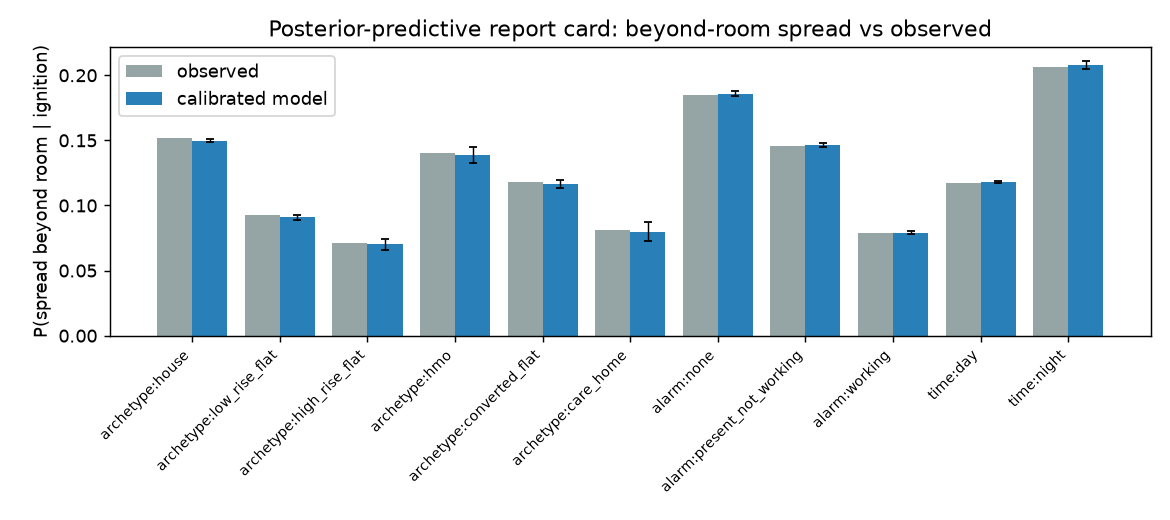
\includegraphics[width=0.49\linewidth]{figures/fig_report_card_room.png}
  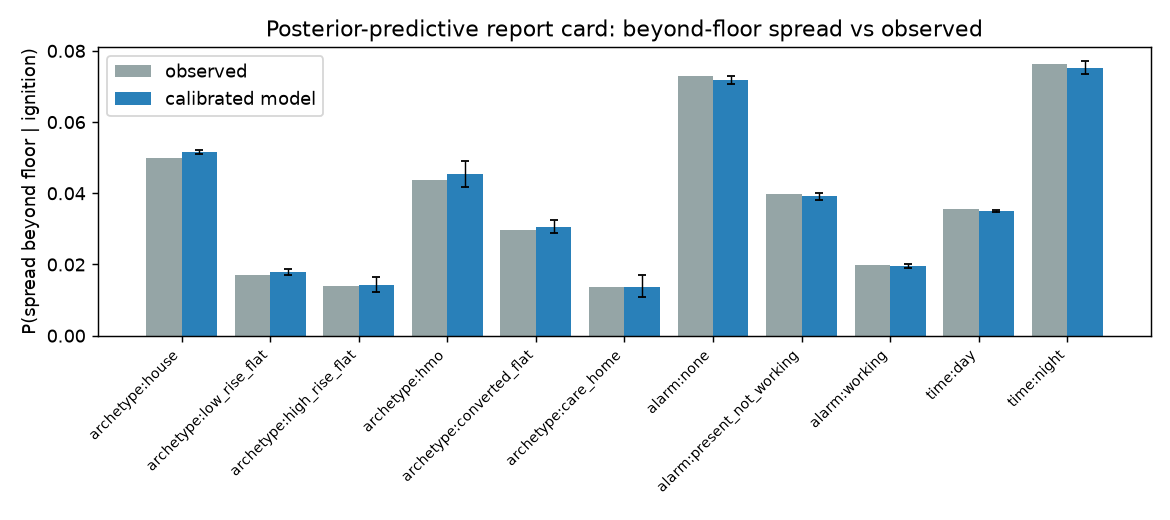
\includegraphics[width=0.49\linewidth]{figures/fig_report_card_floor.png}
  \caption{Posterior-predictive report card: observed spread margins (points)
  vs calibrated-model posterior predictive (intervals), beyond-room (left) and
  beyond-floor (right), all 22 cells.}
  \label{fig:reportcard}
\end{figure}

\subsection{Verdict}

For population-level marginal consequence probabilities, the calibrated engine
can replace the companion framework's stochastic simulator: it matches the same
data while adding physical units, a quantified discrepancy, and the contained-fire
regime the simulator lacks. For per-scenario, timed outputs --- the purpose a
physics engine ultimately serves --- it cannot yet: the driving parameters are
unidentified, beyond-floor spread leans on a discrepancy term twice the size of
beyond-room's, and the tall-shaft regime does not converge. Substituting it
there would trade an honest mechanism for a confounded aggregate fit.

\section{Discussion}
\label{sec:discussion}

Taken together, the two halves of this paper quantify the marginal value of
data granularity on both axes of the companion framework, and the two results
point at the same bottleneck.

\subsection{What national incident data can and cannot identify}
\label{sec:discussion:identify}

The most transferable result of the calibration is not the door-openness value
but the shape of what was learned. Aggregate national spread margins identify
\emph{one} effective degree of freedom of the fire physics --- the
door/ventilation axis --- and leave the growth, heat-release, boundary and yield
parameters prior-dominated (Table~\ref{tab:theta}). We state this positively,
because it is actionable knowledge rather than a mere shortfall: any claim to
have \emph{fully} calibrated a fire-consequence model from national aggregate
incident data should be treated with suspicion, and the analyst who wants the
remaining parameters must go and collect a different kind of data --- the timed,
scenario-resolved outcomes of the axis discussion below --- rather than a larger
volume of the same aggregates. More aggregate margins cannot help, and the
reason is structural, not statistical:

\begin{proposition}[Level sets of the summary map are not updated]
\label{prop:levelset}
Suppose the likelihood depends on the physical parameters $\boldsymbol\theta$
only through a summary map $m:\Theta\to\mathbb{R}^{d}$ --- here the vector of
per-archetype spread margins the emulator returns --- so that
$p(\mathrm{data}\mid\boldsymbol\theta)=g\big(m(\boldsymbol\theta)\big)$ for some
function $g$. Then for any prior $\pi$ and any value $c$ in the range of $m$,
the posterior restricted to the level set
$\{\boldsymbol\theta:m(\boldsymbol\theta)=c\}$ is proportional to the prior
restricted to it; equivalently, prior and posterior induce the same conditional
distribution of $\boldsymbol\theta$ given $m(\boldsymbol\theta)=c$.
\end{proposition}

\begin{proof}
Write $\pi(\boldsymbol\theta\mid\mathrm{data})
= g\big(m(\boldsymbol\theta)\big)\,\pi(\boldsymbol\theta)/Z$ with
$Z=\int g\big(m(\boldsymbol\theta)\big)\,\pi(\boldsymbol\theta)\,
d\boldsymbol\theta$. On the level set $m(\boldsymbol\theta)=c$ the factor
$g\big(m(\boldsymbol\theta)\big)=g(c)$ is constant in $\boldsymbol\theta$, so
there $\pi(\boldsymbol\theta\mid\mathrm{data})=[g(c)/Z]\,\pi(\boldsymbol\theta)$,
a fixed multiple of the prior; after normalisation over the level set the two
densities coincide. If in addition $m$ is smooth, any direction $v$ with
$\nabla m(\boldsymbol\theta)\,v=0$ is tangent to a level set, so moving
$\boldsymbol\theta$ along $v$ leaves the likelihood unchanged; such a direction
can contract from prior to posterior only through the prior's correlation with
the directions on which $m$ actually varies.
\end{proof}

The calibration is this proposition in action. The likelihood reaches
$\boldsymbol\theta$ only through the emulator's predicted margins
$m(\boldsymbol\theta)=\eta(\boldsymbol\theta,\cdot)$, and that map varies
appreciably in essentially one direction (door-openness, the only parameter with
a differential signature across compartmentation-linked cells). The orthogonal
directions lie along level sets of $m$; by the proposition the data cannot move
them, and their posteriors equal their priors up to whatever prior correlation
they carry with the identified axis --- precisely the near-zero contractions of
Table~\ref{tab:theta}. The practical corollary is a data-collection ask, not a
modelling fix: to identify a parameter one must supply a target whose summary map
$m$ actually bends in that parameter's direction, which for fire growth and
heat release means \emph{timed} outcomes, not more spread margins.

\subsection{Marginal value of finer data on both axes}

\paragraph{Spatial axis.} Sub-area concentration is large (24 points above the
density null), predictable (4--6$\times$ out-of-sample targeting multipliers),
and directly monetisable (break-even prevention at small budgets). London is
the demonstration, not the limit: every English fire service records the same
geography internally; only publication practice differs. The record-level
data-sharing route --- the national incident database and its successor ---
would nationalise this result.

\paragraph{Mechanistic axis.} Physics can now be carried through a national
fire-risk framework with calibrated uncertainty --- but aggregate incident
margins buy exactly one physical parameter. Breaking the identifiability
ceiling requires \emph{timed} targets: call-to-arrival and stop times joined to
spread outcomes at incident level, documented case-study timelines, and a small
set of field-model (FDS) anchor runs for the regimes zone models cannot
represent. The first two are data-access questions, not research questions.

\paragraph{Building axis.} Where building identity survives publication (the
care-home slice), building-resolved calibrated inference works today, and
yields observables --- false-alarm burden as alarm reliability --- that the
companion framework's latent-state layer can consume directly. The equity
considerations of risk-targeted prevention discussed in the companion paper
apply with more force as targeting sharpens from areas to cells to buildings;
auditability of the targeting criteria becomes correspondingly more important.

\paragraph{Limitations.} London-only for the spatial results; one-tenure,
regulator-registered stock for the building results; two-zone physics with a
characterised tall-shaft failure and a partially-converged design bank whose
timeout region is mapped but not eliminated; and consequence economics inherited
from national parameters absent cell-level occupancy data. Each is stated where
it binds.

\section{Conclusion}

Fire risk in English dwellings is concentrated well below the geography at
which the country records it, predictably enough to raise the value of a fixed prevention budget four- to
sixfold; building-resolved calibrated inference is
already possible wherever building identity is published; and zone-model
physics can be statistically calibrated against the national incident record
--- to a precisely characterised ceiling. The common denominator is data
resolution, not method: the framework, the economics, and now the physics are
ready for finer targets than the public record currently provides.

\appendix
\section{Methods summary (companion-paper definitions used here)}
\label{app:methods}

\paragraph{Spread margins.} The calibration targets are the observed marginal
probabilities, over 451{,}172 record-level English dwelling fires
(2010/11--2024/25), of fire spread \emph{beyond the room of origin} and
\emph{beyond the floor of origin}, computed by archetype-mapped dwelling type,
alarm state (absent / present-not-operated / operated), and time of day ---
22 cells in all, each with its count denominator.

\paragraph{Archetypes.} Seven parameterised room--corridor--stair graph
families (detached and terraced houses, low- and high-rise purpose-built
flats, HMO, care-home wing, mixed-use residential-over-commercial); rooms carry
type, area (EPC-informed), and occupants; edges carry a barrier class (open /
internal door / fire door / compartment wall) with open-state probabilities.
The CFAST translation maps rooms to compartments, barriers to vents, and
construction era to effective single-layer boundary conduction properties.

\paragraph{Design fires.} $t^2$ growth to a peak HRR with class-specific
growth constants and soot/CO yields: cooking (medium growth, 1--3\,MW),
upholstered/smoking (slow--medium), electrical wiring (slow),
battery/charger (fast; wide prior), candles (medium); class weights follow the
national ignition-source distribution.

\paragraph{Prevention economics.} \pounds55 per visit; averted value =
posterior fire rate $\times$ P(no working alarm) $\times$ (casualty channel:
base casualty rate $\times$ interventional relative risk reduction $\times$
\pounds66{,}113 + property channel: \pounds2{,}802), discounted over a
10-year alarm life at 3.5\% (present-value multiplier 8.61). All values and
their provenance (Home Office \emph{Economic and Social Cost of Fire} 2023
sheets; stated-assumption tags) follow the companion paper.

\IfFileExists{repro_appendix.tex}{\section{Reproducibility}
\label{app:repro2}

Every numbered figure and table in this paper traces to a results artifact under
\texttt{results/}, produced by a module under \texttt{src/} that reads the project
database. The end-to-end map, the environment (\texttt{requirements.txt}, frozen
versions; Python~3.12, plus \texttt{gfortran} to build NIST CFAST for the physics
engine), and the one-command database rebuild
(\texttt{python -m src.build\_db --with-epc --with-lfb}, or attach the shipped
DuckDB files) are documented in \texttt{REPRODUCE.md} at the repository root.
Priors are exactly as stated in the model and calibration sections; all sampler
settings (draws, warmup, chains, design sizes) live in the cited modules and are
echoed into each \texttt{results/*/summary.md} or \texttt{report.md}. All Monte
Carlo, MCMC and Latin-hypercube runs use fixed seeds, listed below.
Tables~\ref{tab:repro-fig2} and~\ref{tab:repro-tab2} give the per-figure and
per-table provenance; the sub-LSOA maps use live basemap tiles and so may render
cosmetically differently, as noted in \texttt{REPRODUCE.md} \S7.

\begin{table}[htbp]
  \centering
  \small
  \setlength{\tabcolsep}{4pt}
  \caption{Reproducing each numbered \emph{figure}. Commands are run from the
  repository root inside the virtual environment.}
  \label{tab:repro-fig2}
  \begin{tabular}{@{}p{1.5cm}p{4.5cm}p{4.1cm}p{4.1cm}@{}}
    \toprule
    Figure & Producing module / function & Input artifacts & Seed(s) \& config \\
    \midrule
    \ref{fig:concentration} & \texttt{src.models.london\_pilot}
      (\texttt{fig\_concentration}) & London 50\,m cell panel
      (\texttt{results/london\_pilot/}) & \texttt{SEED=20260706} \\
    \ref{fig:map} & \texttt{python src/viz/build\_map\_2x2.py}
      (\,+\,\texttt{build\_map\_inset.py}) & \texttt{data/processed/london\_map\_cells.parquet};
      live CARTO/OSM tiles & no seed (basemap live) \\
    \ref{fig:targeting} & \texttt{src.models.london\_pilot} (\texttt{fig\_targeting})
      & \texttt{results/london\_pilot/} targeting economics
      & \texttt{SEED=20260706} \\
    \ref{fig:carehome} & \texttt{src.models.london\_pilot}
      (\texttt{fig\_carehome\_rates}, analysis~B) & care-home building panel
      (\texttt{results/london\_pilot/}) & \texttt{SEED=20260706} \\
    \ref{fig:reportcard} & \texttt{src.physics.phaseB\_analysis}
      (\texttt{fig\_report\_card}) & calibration posterior
      (\texttt{results/physics/calibration/posterior.nc})
      & calibrate \texttt{PRNGKey(0)}, NUTS $4\times(1000{+}1000)$ \\
    \bottomrule
  \end{tabular}
\end{table}

\begin{table}[htbp]
  \centering
  \small
  \setlength{\tabcolsep}{4pt}
  \caption{Reproducing each numbered \emph{table}.}
  \label{tab:repro-tab2}
  \begin{tabular}{@{}p{1.6cm}p{4.6cm}p{4.0cm}p{4.0cm}@{}}
    \toprule
    Table & Producing module / command & Input artifacts & Seed(s) \& config \\
    \midrule
    \ref{tab:concentration} & \texttt{python -m src.models.london\_pilot}
      & \texttt{results/london\_pilot/summary.md} & \texttt{SEED=20260706} \\
    \ref{tab:cellvalue} & \texttt{python -m src.models.london\_pilot}
      (\texttt{targeting\_economics}) & \texttt{results/london\_pilot/}
      ranked-cell value & \texttt{SEED=20260706} \\
    \ref{tab:boroughs} & \texttt{python src/viz/build\_borough\_table.py}
      & \texttt{results/london\_pilot/borough\_allocation.csv}
      & deterministic from ranked cells (no seed) \\
    \ref{tab:theta} & \texttt{python -m src.physics.calibrate} then
      \texttt{src.physics.phaseB\_analysis} (\texttt{behavioural\_table})
      & CFAST sweep emulator; \texttt{posterior.nc}
      & sweep \texttt{seed=20260706}; calibrate \texttt{PRNGKey(0)},
      NUTS $4\times(1000{+}1000)$, LHS $M{=}1400$ \\
    \bottomrule
  \end{tabular}
\end{table}
}{}

{\small
\setlength{\columnsep}{18pt}
\begin{multicols}{2}
\bibliographystyle{plainnat}
\bibliography{references}
\end{multicols}
}

\end{document}
